\section{Introduction}
When working with machine learning models, it becomes very important to be aware of the implications that the hardware and technical limitations can have in the model training, architecture selection, memory and computational cost. In the research paper Numerical influence of ReLU’(0) on backpropagation \cite{ORIGINAL} that we are reproducing, one of the main arguments is the difference between the theoretical (not limited in precision) and technical capabilities of a model. In theory, there's no memory or bit-precision, nevertheless, computational limitations must be taken into account when training the model. We also run additional experiments to further extend the authors' idea of the value of the subgradient being a hyperparameter to tune during training.

\section{Scope of reproducibility}
\label{sec:claims}

The original paper \cite{ORIGINAL} states that when using a 32 and 16-bit precision for the tensor storage and computation, the bifurcation zone (i.e. the set $S_{0,1}$ of weights such that $backprop_0 \neq backprop_1$ for two identically initialized and trained models) is met with non-null probability. The choice of ReLU'(0) becomes computationally meaningful and influences the training and test accuracy. As the trend to lower the precision to make the model training more efficient in terms of energy, memory and resources are arising, it was very important for us to understand and make sense of the implications of changing the value of ReLU'(0) in practice. The main takeaway from the original paper is that the arbitrary choice of mathematically negligible factors (such as the ReLU'(0)) might not be computationally negligible. Nevertheless, the author's conclusion is that ReLU'(0) = 0 (which is what is conventionally used both in theory and in the major deep learning frameworks) seems to be the most robust selection for training across the variations the original authors tried. Given our goal to see the influence of such choices where low precision might be meaningful, we run our tests on both simple and more complex models, including MobileNet V3 small \cite{MOBILENETV3}: a model engineered to work in low resources use-cases. One of the main motivations is that as models become bigger and more complex, errors due to numerical precision happen with relatively high frequency. Additionally, the necessity of using smaller bit-precision increases with tighter memory, time, and energy constraints. In the academic case, it is also interesting to use lower precision because it helps with improving resource usage. Our objectives then were to understand the theoretical background, the potential influence on the practical scope, and if there's room to take advantage of this peculiarity.

To achieve that, we first reproduced\footnote{\url{https://anonymous.4open.science/r/ml-reproducibility-challenge-5D70/README.md}} the experiments to support the main claims of the original paper (detect and measure the difference on fully connected networks trained with different values for ReLU'(0)), then we tried to use the subgradient as a hyperparameter during tuning to see if we could reach better performance (measured as the accuracy on the validation set).

\section{Methodology}
Given the existing codebase from the original paper\footnote{\url{https://github.com/deel-ai/relu-prime}}, our approach consisted in applying a similar approach to the authors' and adapting part of the existing implementations to suit our goals. Nevertheless, the vast majority of the experiments and codebase have been redesigned, so that we could get a better understanding of the procedure and properly explain the results and make additional explorations (such as hyperparameter tuning). Tools we used include Kaggle cloud services as well as our personal devices with GPUs that didn't allow us to run large models or a large number of experiments. The first results were reproduced as we first needed to see if the code was properly implemented. Once the results were consistent, we started to think about reproducing results with different architectures, optimisers, normalizations, and activation functions (with at least one non-differentiable point).

\subsection{Model descriptions}
We investigate the influence of the subgradient hyperparameter in different architectures to see if the findings could be relevant to a broader spectrum of models. In particular, we run our tests on the following models:

\begin{itemize}
\item Fully connected NN (with different widths and depths)
\item ResNet-18
\item MobileNet V3
\end{itemize}

We chose the fully connected architecture because of its flexibility, and customizability, and because it is densely packed with ReLU activations so the effect can be easily analyzed. We are also trying to maintain enough similarities with the original paper so we can compare the results. The ResNet-18 and MobileNet V3 were chosen to investigate the effect on CNNs with residual blocks and inverted residual blocks respectively. Additionally, the MobileNet V3 mixes ReLU activations (or ReLU6) with Hardsigmoid ones, which further increases variability.

\subsection{Datasets}
In order to reproduce the paper without the need to have a complex model and data set that could take much to train, we decided to work with the MNIST dataset. The MNIST\footnote{\url{http://yann.lecun.com/exdb/mnist/}} (and its variation FashionMNIST\footnote{\url{https://github.com/zalandoresearch/fashion-mnist}}) dataset allowed us to run manageable experiments given our computational and storage constraints. Moreover, according to our goals, it was enough to start with it and possibly extend the experiments to a more complex data set. Both datasets consist of both a 60000-sample training set and a 10000-sample test set. Each element is a 28x28 greyscale image, this means that we just have one channel per image and 784 pixels in total. However, MobileNet V3 is built to work with 3-channels input, so transforming the grayscale image into a 3-channel RGB image with the same grayscale value for each channel was necessary.

\subsection{Hyperparameters}
As stated in the original paper and as seen in our experiments, the value of ReLU'(0) can become a hyperparameter to tune. We run the initial experiments both in 32-bit and 16-bit precision to compare the influence of numerical precision on the size of the bifurcation zone. We decided not to run them in 64-bit precision as well because, as evidenced in the original paper as well, it is less likely to have numerical errors and therefore a rounding to exactly 0 in the forward pass, and hence to observe an influence by the choice of ReLU'(0) value. In summary, the most important hyperparameters to choose were the following:
\begin{itemize}
\item Precision: 16 or 32-bit precision 
\item Model architecture
\item Activation function: ReLU vs ReLU6 (vs LeakyReLU)
\item Value of the subgradient in the non-differentiable point(s)
\item Batch Size
\end{itemize}

For all experiments, we used the ADAM optimizer with a 0.001 learning rate, and for most experiments we used a fixed batch size of 128. 

\subsection{Computational requirements}
This work studies the effect of the subgradient in the backpropagation step, thus we needed to compute several models with different subgradients using PyTorch. We ran the experiments using Python 3.9.12 and PyTorch 1.13.1 with CUDA 11.7. We ran the experiments using Kaggle, Google Colab and local GPUs	(Nvidia GeForce RTX 3060).

\section{Results}
\label{sec:results}
We selected some of the experiments that we found most meaningful to reproduce, because of computational constraints and our focus on estimating the impact of the subgradient choice, mainly through the weight difference (or $L_1$ norm between the weight matrices), the volume of the gradient matrix in the backpropagation (comparison of differences in the gradients) and the performance of the models with both training and testing losses.

\subsection{Initial Experiment} 

The first step was to compare the weight difference of the parameters with both 32 and 16-bit precision models and check the bifurcation zone, to see when and why they start to diverge. What we did here was to train two models that differ only in the subgradient choice and measure the $L^1$ norm between their weight matrices to have a perception of how different they became. This part does not measure whether a solution is better than the other, but it helps us to understand the magnitude of the change. This is one important point because it explains the importance of the experiments performed in this paper. We can observe that even with 32-bit precision we can notice a small difference in performance (validation accuracy), depending on the election of the ReLU'(0), and the effect is indeed greater using 16-bit precision. Therefore, it turns reasonable and interesting to analyze how the choice of ReLU'(0) impacts the difference and which of the values in the interval [0,1] is more desirable. We notice, however, as can be seen in figures \ref{fig:asdf} (a) and (b) that the lower the precision is more unstable, and the weight difference between them varies rapidly because the exact activation value of zero is reached more frequently.

\begin{figure}[htbp]
    \centering
        \subfigure(a){\includegraphics[width=0.4\columnwidth]{Images/Init_32.png}} 
        \subfigure(b){\includegraphics[width=0.4\columnwidth]{Images/Init_16.png}} 
    \caption{(a)  $|\theta_0 - \theta_1|_1 $with 32-bit precision. (b) $|\theta_0 - \theta_1|_1$ with 16-bit precision. }
    \label{fig:asdf}
\end{figure}

\subsection{Fully connected Neural Network} 

After we observed the first results with the functions we implemented, and confirmed that they were consistent with the paper, we decided to run the experiments with a fully connected neural network. Some hyperparameters were the same for all the experiments, we just changed the value of $ReLU'(0) \neq 0$ in different bit precision to observe if there were any changes in loss and accuracy of the models with this difference and to measure them on similar conditions. 
The hyperparameters that we decided to fix were: 
\begin{itemize}
\item Number of epochs: 50
\item Optimizer: ADAM with our default learning rate
\item Number of layers: 3
\item Nodes in hidden layers: 200
\item Regularization: Not used for this experiment (Identity)
\end{itemize}

With these hyperparameters fixed, the values for the subgradient we used were: $ReLU'(0) = [ 0, -0.5, 0.5, 0.8, 1 ]$.

%%%%%%%%%%%%%
\subsubsection{Results with 32-bit precision}


When comparing the sum of the weights, we could immediately observe that the use of $ReLU'(0) \neq 0$ does have a big effect on the weights. They start to have different magnitudes, and the difference becomes bigger. Nevertheless, that does not mean the accuracy must be worse, as we could be getting to a different but equally-good local minimum of the problem. 

\begin{figure}[hbtp]
    \centering
        \subfigure(a){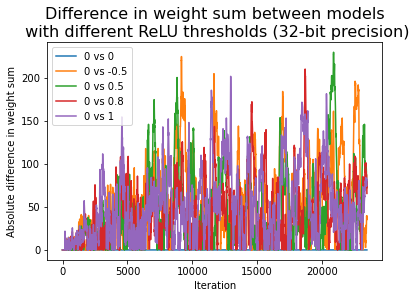
\includegraphics[width=0.4\columnwidth]{Images/WeightSum32.png}} 
        \subfigure(b){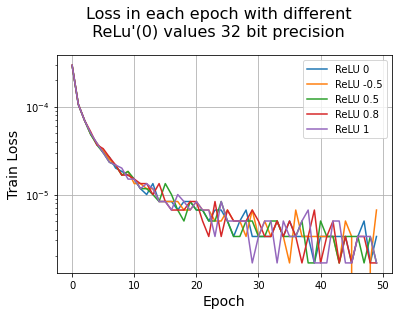
\includegraphics[width=0.4\columnwidth]{Images/LossTrain32.png}} 
        \subfigure(c){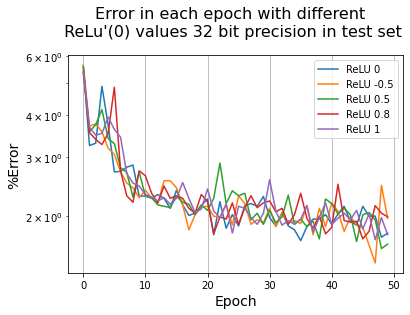
\includegraphics[width=0.4\columnwidth]{Images/ErrorTest32.png}}
        \subfigure(d){\includegraphics[width=0.4\columnwidth]{Images/WeightSum16.png}} 
        \subfigure(e){\includegraphics[width=0.4\columnwidth]{Images/LossTrain16.png}} 
        \subfigure(f){\includegraphics[width=0.4\columnwidth]{Images/ErrorTest16.png}}
    \caption{(a)   $|\theta_0 - \theta_1|_1$ with 32-bit precision and different $ReLU'(0)$ values (b) Training loss of the model with different subgradients  (c) Test Loss of the model with different subgradients. \\
    (d)   $|\theta_0 - \theta_1|_1$ with 16-bit precision and different $ReLU'(0)$ values (e) Training loss of the model with different subgradients  (f) Test Loss of the model with different subgradients.}
    \label{fig:validation32}
\end{figure}

For the training loss, we observe that with 32-bit precision there's no big difference, even though the weights are very different in magnitude, which indicates that even with those subgradients, the solution converges. However, the value of $ReLU'(0) = 0$ looks more stable, but the low number of epochs might not be enough to see if it eventually becomes more chaotic. Figure \ref{fig:validation32} shows the performance on the training and test set. 




%%%%%%%%%%%%%%%%%


\subsubsection{Results with 16-bit precision}


With 16-bit precision, it becomes evident that we should be considering the value of $ReLU'(0) $ when training, and it becomes important the chose of $ReLU'(0) = 0$ as a correct decision. With other values, the behaviour becomes chaotic both for training and validation. 

Firstly, we can observe that the values of the weights become different with a logarithmic behaviour, but it was also imperative to test whether this was just getting to different but accurate solutions to the problem. The next step was to see the training loss and check whether the solutions were accurate, and if so, determine the impact of $ReLU'(0) $. When inspecting the plot, we can observe that the behaviour becomes very chaotic and the larger the values, the faster it would diverge from the solution. It would be also interesting to see if could change with different learning rates or optimizers. After this experiment, we proceeded to validate the model with the test data set, which resulted in the same behaviour. Lastly, we decided to compare the distribution of the test accuracy. This was a good way to compare the performances of each model with different values (see figure \ref{fig:foobar}).  

\begin{figure}[htbp]
    \centering
        \subfigure{\includegraphics[width=0.5\linewidth]{Images/Accuracy.png}} 
    \caption{ Comparison between model accuracies using box-plots, this allows us to look at the distribution of the accuracy through all the experiments}
    \label{fig:foobar}
\end{figure}

It became evident that not only the accuracy is worse depending on the value of the subgradient, but it's also less stable, the standard deviation gets bigger with the value of $ReLU'(0)$ which is an indicator that for this model the most robust election is the value of $ReLU'(0) = 0$.

\subsection{Volume measurement}

Other important point was to have a notion of how the weights were changing the more complex the model became. To understand this, we decided to get the volumes for fully connected models, as was done in the paper. In this case, we needed to make smaller models due to limitations in computing resources. Nevertheless, even at a smaller scale, we could observe similar tendencies. For this experiment, there were several variations. But through all of them, the two models have fixed subgradients.

\begin{itemize}
\item Model 1 : $ReLU'(0) = 0 $
\item Model 2 : $ReLU'(0) = 1$
\end{itemize}

It's important to note that in this experiment we do not do the hyperparameter tuning step, as it's not the objective to measure the performance of the model but the difference between the gradient matrices, which can indicate how different the models are and how many zeros we have when changing the parameters. 

\begin{figure}[htbp]
    \centering
        \subfigure(a){\includegraphics[width=0.4\columnwidth]{Images/Layers.png}} 
        \subfigure(b){\includegraphics[width=0.4\columnwidth]{Images/Neurons.png}} 
        \subfigure(c){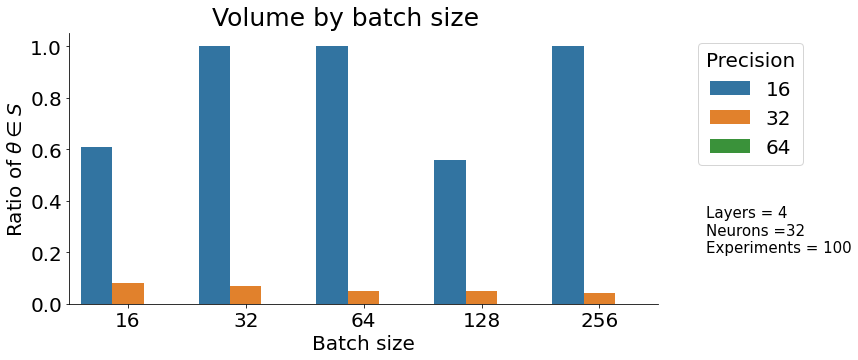
\includegraphics[width=0.4\columnwidth]{Images/Batch.png}}
        \subfigure(d){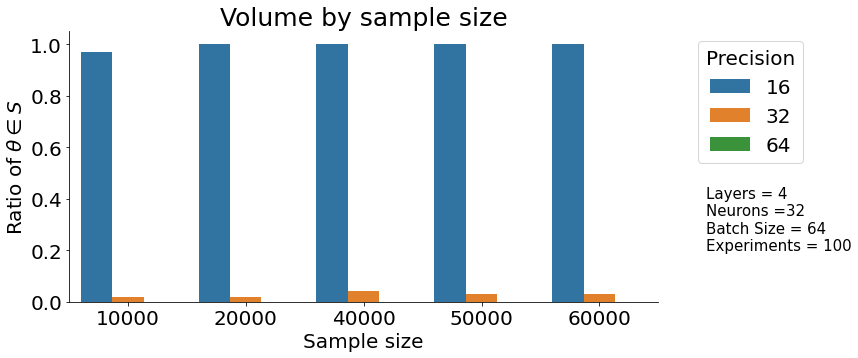
\includegraphics[width=0.4\columnwidth]{Images/Sample}}
    \caption{The volume of the model weights was a measurement of the difference between the gradient matrices (a) Comparison by varying the number of layers   (b) Comparison by varying the number of neurons by layer (c) Comparison by varying the number of batch sizes for the forward and backward pass (d) Comparison by varying the number of samples from the dataset. }
    \label{fig:Volumes}
\end{figure}

The first experiment was to iterate with different depths or the number of layers. We used 64, 32 and 16-bit precision so that we could better compare the results. We used the 64-bit precision experiment as our reference. In figure \ref{fig:Volumes} (a) we see that the deeper the model, the higher the probability of getting a value of 0 at the ReLU point with the 16 and 32 precision, at 16 bit this becomes much more relevant as we can see that the gradient matrix start to become much different even in small layers. With 32-bit (PyTorch default value) the difference is not heavily impacted by the model depth. We observe a similar behaviour with the number of neurons per layer. The more neurons, the more likely that a value can become 0. And again, this probability is much higher for the 16-bit precision. For the sample size and batch size, we could observe a difference with 32-bit precision but it was not significant and there is not much variation, whereas at 16-bit precision it still very significant even with batch and sample sizes.  


\subsection{ResNet18}
\label{ResNet18}

To study the generalization across model architectures, we reproduced the experiments with ResNet18, a Convolutional Neural Network with Residual Blocks. The model also has layers that use batch normalization. In the original paper, the authors ran experiments using batch normalization, and the results were that it stabilizes the weight matrices. We wanted to put this to the test and run it with different subgradient values to measure the behaviour of the models and see if for this for more complex models this difference could be much significant. We decided to use this specific structure as it does not have an excessive amount of layers, so it is feasible to work with it, but has an excellent and representative functionality, thus it is a good option to evaluate the desired outcome. In this case, as the architecture is fixed, the only parameter we changed was the value used at ReLU'(0), where we tested the same set we employed in the previous analysis $ ReLU'(0) = [ 0 , -0.5 , 0.5 , 0.8 , 1 ]$.

The hyper parameters that we decided to fix were: 

\begin{itemize}
\item Number of epochs:20
\item Optimizer: ADAM with our default learning rate. 
\item Regularization: Batch normalization (built-in in the model)  
\end{itemize}

We could run the experiments with 32-bit precision, and the results were consistent with the paper's claims. When adding batch normalization in each layer, the model became much more stable. This was perhaps because there were not many values getting to 0. 

\begin{figure}[hbtp]
    \centering
        \subfigure(a){\includegraphics[width=0.45\columnwidth]{Images/RN_weight_32.png}} 
        \subfigure(b){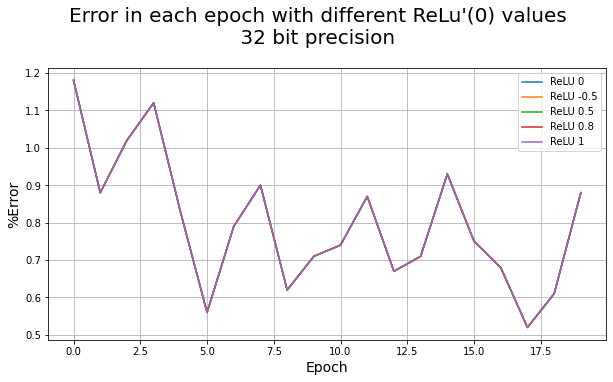
\includegraphics[width=0.4\columnwidth]{Images/ResN18_Test.png}}
    \caption{(a) The $L_1$ norm of the weights w.r.t the ReLU'(0) (b) The test error in the different models }
\end{figure}

Something interesting when ruining it with the 32 bit precision, was that the model was very stable with any subgradiant value. Which indicate us that this model is very stable thanks to batch normalization and that many weights might not get to the ReLU(0) value. We were not able to complete the 16-bit precision tests for this model due to execution problems, though we could see how stable it was with 32-bit precision. When comparing it with a fully connected neural network it becomes evident.

\subsection{MobileNet V3}

Reproducing the initial experiment with MobileNet and ReLU as the activation function led to no differences detected in the first 2 training epochs as can be seen in our repository. However, we used MobileNet to see if the idea of using the value of the subgradient could be actually used as a real hyperparameter in a hyperparameter tuning process.
To do that, we used Ray tune which allowed us to do the random grid search in the hyperparameter space and checkpoint the models.

To run the experiments we chose:

\begin{itemize}
\item Number of epochs: 6 (due to computational power limit)
\item Optimizer: ADAM 
\item Activation function: ReLU6 (two non-differentiable points \textit{alpha} and \textit{beta})
\end{itemize}

The hyperparameter space we set for the experiment included:

\begin{itemize}
\item Batch size: choice [32, 64, 128]
\item ADAM learning rate: loguniform [1e-4, 1e-2] 
\item \textit{alpha} and \textit{beta}: uniform [0, 1]
\end{itemize}

The most promising model we obtained has reached 96.9167\% accuracy with a cross-entropy loss of 0.101213 by using a batch size of 64, a learning rate of 0.00170239, \textit{alpha} = 0.496422, and \textit{beta} = 0.455249. The model performs worse than the best model obtained excluding \textit{alpha} and \textit{beta} from our search space (accuracy: 97.3583\%, cross-entropy loss: 0.0869832, batch size: 64, learning rate: 0.0031722)

The results are coherent with the findings above. Although the low number of epochs, a different choice for the subgradient in both non-differentiable points induces a chaotic behaviour that makes the solution less stable and precise. Even trying to further train the best models for more epochs and using a smaller learning rate leads to the same result, with the default choice of ReLU6'(0) = ReLU6'(6) = 0 being the more appropriate.

\begin{figure}[hbtp]
    \centering
        \subfigure(a){\includegraphics[width=0.45\columnwidth]{Images/mobilenet_hyperparameter_tuning_train.png}} 
        \subfigure(b){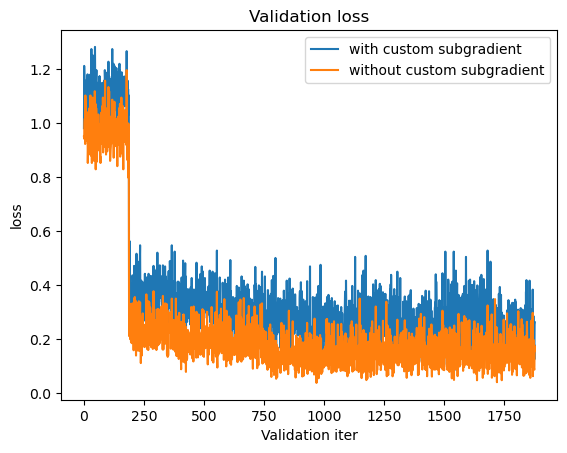
\includegraphics[width=0.45\columnwidth]{Images/mobilenet_hyperparameter_tuning_val.png}}
    \caption{(a) Train loss while training the two best models (including and excluding \textit{alpha} and \textit{beta} as hyperparameters) (b) The validation error }
\end{figure}

We ran the same hyperparameter tuning process on the fully connected model, and our results were coherent with the whole analysis above (see our repository). However, we noticed that when training the model with a customized value of the subgradients the non-differentiable points are reached less frequently as the training goes on, while training without the default subgradient the non-differentiable points are hit more frequently.

\section{Summary}

The subgradient is a surrogate of the derivative in a non-differentiable point of a non-smooth function. In theory, it wouldn't matter the value it takes as long as is within the slope of the two functions that define the function, in the case of the ReLU function it is between 0 and 1. Even though in theory this is correct, when using numerical methods to perform a backpropagation, altogether with numerical bit-precision it becomes relevant as rounding errors can lead to different solutions. As the use of 32-bit precision is widely used as a standard in neural network training and as 16-bit is becoming a trend to speed up the training in GPUs and energy saving, the choice of subgradient becomes relevant. Although 0 seems to be an adequate election, it becomes a hyperparameter when training and testing the model. These experiments and results can be used as a solid base to keep the election of the subgradient $ReLU'(0)=0$ when training a model at 16 and 32-bit precision.